\subsubsection{usergoal-ugPassRecovery}

\label{RE-use-case-ugPassRecovery}




\begin{usecase}
  \addheading{Use-Case Description}
  \addsingletwocolumnrow{Name}{ugPassRecovery}
  \addsingletwocolumnrow{Scope}{system}
  \addsingletwocolumnrow{Level}{usergoal}
  

\addrowheading{Primary actor(s)}
\addnumberedsinglerow{}{\msrcode{actAdministrator[active]}}



\addrowheading{Goal(s) description}
\addsinglerow{}


\addrowheading{Protocol condition(s)}
\addnumberedsinglerow{}{
}

\addrowheading{Pre-condition(s)}
\addnumberedsinglerow{}{
}

\addrowheading{Main post-condition(s)}
\addnumberedsinglerow{}{
}

\addrowheading{Main Steps}
\addalphanumberedsinglerow{}{the actor \msrcode{actAdministrator} executes the \msrucname{oeLoginRecov} use case}
\addalphanumberedsinglerow{}{the actor \msrcode{actAdministrator} executes the \msrucname{oeUpdatePass} use case}
\addalphanumberedsinglerow{}{the actor \msrcode{actAdministrator} executes the \msrucname{oeLogin} use case}
\addalphanumberedsinglerow{}{the actor \msrcode{actAdministrator} executes the \msrucname{oeLogout} use case}
\addrowheading{Steps Ordering Constraints}
\addnumberedsinglerow{}{step(b) is possible after step(a)}
\addnumberedsinglerow{}{steps (a) and (b) can be executed multiple times.}

\addrowheading{Additional Information}
\addsinglerow{
none
}

\end{usecase} 


Figure \ref{fig:lu.uni.lassy.excalibur.examples.icrash-RE-UCD-uc-ugPassRecovery}

\begin{figure}[htbp]
\begin{center}

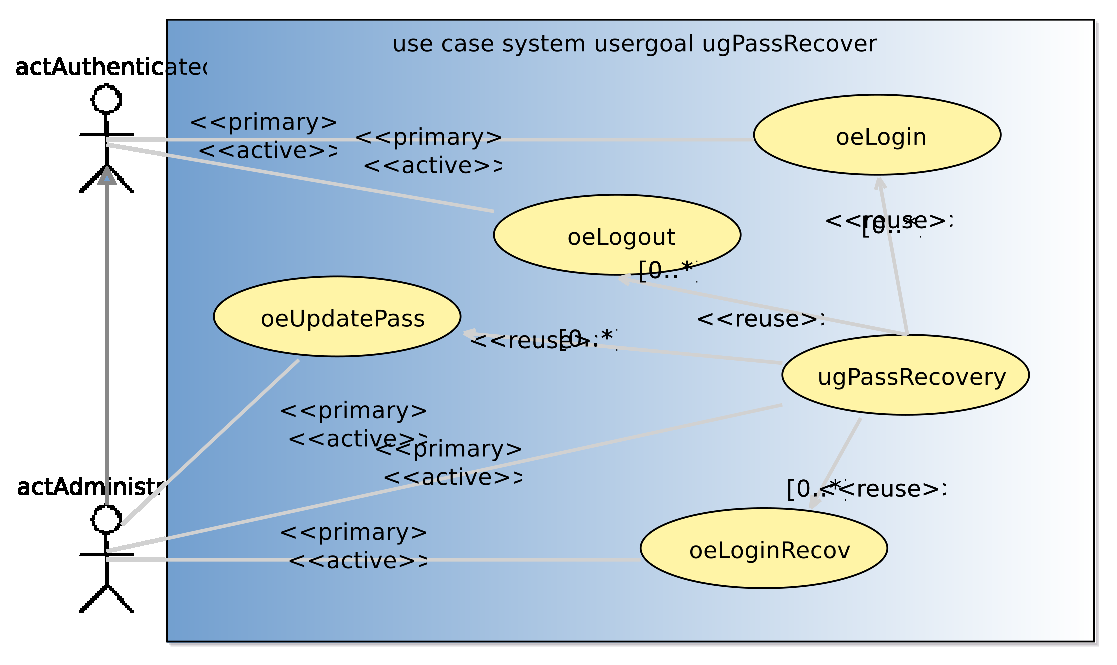
\includegraphics[
angle=0
]{./images-report-gen/usecase-model/usergoal/uc-ugPassRecovery.eps}
\end{center}
\caption[lu.uni.lassy.excalibur.examples.icrash Use Case Diagram: uc-ugPassRecovery]{}
\label{fig:lu.uni.lassy.excalibur.examples.icrash-RE-UCD-uc-ugPassRecovery}
\end{figure}
\vspace{0.5cm}
